\Chapter{Inleiding}

 In dit inleidende hoofdstuk zal enige achtergrondinformatie verschaft worden omtrent cryptografie. Verder wordt het concept identiteitsgebaseerde cryptografie duidelijk gemaakt. Er zal uitgelegd worden waarom de recente ontdekking van het constructieve gebruik van paringen hier zo belangrijk voor is. Ten slotte geeft een kort overzicht aan wat in de literatuur terug te vinden is qua implementaties van paringen. In het volgende hoofdstuk wordt de werking van paringen dan wiskundig uitgespit.

\section{Basisachtergrond cryptografie}

Sinds het begin der tijden is er een nood geweest aan manieren om berichten versleuteld te verzenden tussen twee partijen. Voorbeelden van enkele klassieke encryptiemethoden zijn het Atbashcijfer~\cite{athbash} (Babyloni\"e, 600 v.\ Chr.), het Caesarcijfer~\cite{caesar} (Rome, 56 n.\ Chr.) en het dubbele transpositiecijfer~\cite{kahn} (o.a.\ gebruikt door weerstandsgroepen in WO II). E\'en eigenschap die al deze methodes met elkaar gemeen hebben, is het gebruik van dezelfde sleutel voor versleutelen en ontcijferen. Ook vele moderne encryptiemethodes, zoals bijvoorbeeld 3DES~\cite{3des} en AES~\cite{aes}, gebruiken dit principe, dat men symmetrische versleuteling noemt.

In \reffig{fig-encryptie-applicaties-sym-cipher} wordt de algemene werking van een symmetrische encryptie getoond. Alice zendt een bericht M naar Bob, vercijferd met een door hen beiden gekende sleutel $k$. Bob op zijn beurt ontcijfert met diezelfde sleutel de cijfertekst C. Indien Eve de vooraf afgesproken sleutel kent, kan zij alle communicatie tussen Alice en Bob ontcijferen. Er is dus nood aan een manier om veilig een sleutel $k$ af te spreken tussen twee partijen.

\begin{figure}[h]
	\centering
		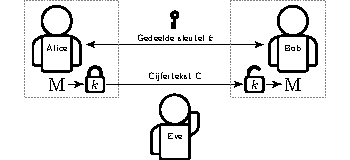
\includegraphics[scale=1.4]{symmetric-cipher-model}
		\caption{Algemene werking van symmetrische encryptie\label{fig-encryptie-applicaties-sym-cipher}}
\end{figure}

Een oplossing voor het veilig afspreken van een gedeelde sleutel was tot 1976 niet gekend. Toen stelden Diffie en Hellman hun algoritme voor sleuteluitwisseling over een onbeveiligd kanaal voor \cite{diffie-hellman}. Deze ontdekking plaveide de weg voor asymmetrische cryptografie (ook wel publieke sleutel cryptografie genoemd). Met behulp van dit type cryptografie kunnen eveneens boodschappen versleuteld worden. Dit wordt ge\"illustreerd in \reffig{fig-encryptie-applicaties-asym-cipher}. Wanneer Alice een bericht M naar Bob wil versturen, zoekt ze eerst zijn publieke sleutel $k_P$ op in een databank. Vervolgens versleutelt ze haar bericht met die publieke sleutel. Enkel Bob kan met behulp van zijn geheime sleutel $k_G$ dan het bericht ontcijferen. Een systeem als dit biedt het grote voordeel dat er geen nood is om de gebruikte (publieke) sleutel geheim te houden. Het is namelijk onmogelijk om met de publieke sleutel de cijfertekst te ontcijferen. Eve heeft er in dit geval dus geen baat bij de gebruikte publieke sleutel te onderscheppen. 

\begin{figure}[h]
	\centering
		 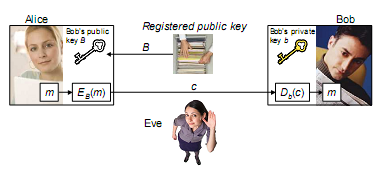
\includegraphics[scale=1.4]{asymmetric-cipher-model}
		 \caption{Algemene werking van asymmetrische encryptie\label{fig-encryptie-applicaties-asym-cipher}}
\end{figure}

Een andere toepassing van asymmetrische cryptografie is het plaatsen en verifi\"eren van digitale handtekeningen. Digitale handtekeningen zijn vergelijkbaar met klassieke handtekeningen. Ze kunnen, indien juist ge\-\"im\-ple\-men\-teerd, gebruikt worden om te verifi\"eren dat een bepaald bericht effectief door de persoon verstuurd is die de verzender beweert te zijn. Ook kan men aan de hand van een digitale handtekening nagaan of de inhoud van een bericht niet gewijzigd werd door een derde persoon tijdens de verzending. ECDSA \cite{ecdsa} en RSA \cite{rsa} zijn enkele van de vele cryptografische algoritmes die toelaten digitale handtekeningen te genereren.

Om te verzekeren dat de publieke sleutels van elke mogelijke ontvanger voorradig zijn, dient een soort een centrale databank voorzien te worden. Indien iemand het voor anderen mogelijk wil maken hem versleutelde berichten te versturen, genereert die persoon eerst een publieke en een private sleutel. De publieke sleutel wordt vervolgens naar de database gestuurd, waar iedereen hem kan ophalen.

\section{Identiteitsgebaseerde cryptografie}

Een nadeel van de publieke sleutel cryptografie zoals voorgesteld in de vorige paragraaf zit hem in het sleutelbeheer. Er is geen manier om zeker te zijn dat, wanneer de publieke sleutel van Bob opgevraagd wordt, de verkregen sleutel effectief die van Bob is. Indien Eve bijvoorbeeld haar publieke sleutel in de database laat opslaan onder Bobs naam, zal Alice berichten voor Bob versleutelen met Eves publieke sleutel. Een mogelijke oplossing hiervoor is bijvoorbeeld het ``web of trust'', zoals ge\"implementeerd door de software PGP \cite{pgp}. Daarbij kunnen mensen aangeven of ze een bepaalde publieke sleutel betrouwbaar vinden of niet. Een sleutel die vergezeld wordt van meerdere getuigenissen van betrouwbaarheid zal dat dan waarschijnlijk ook zijn. Verder bestaat er een zogenaamde ``revocation list'', die aangeeft welke sleutels niet meer geldig zijn.

Uiteraard is ook zo een systeem niet volledig waterdicht. Iemand kan bijvoorbeeld onder verschillende identiteiten sleutels insturen en vervolgens, met al die verschillende identiteiten, zijn sleutels een certificaat van vertrouwen geven. Indien iemands publieke sleutel zou afgeleid kunnen worden van bekende gegevens omtrent zijn identiteit, dan zouden deze problemen niet bestaan.

In 1984 stelde Shamir een methode voor waarbij dit mogelijk zou zijn \cite{shamir}. Het basisidee is als volgt: in plaats van een centrale databank voor publieke sleutels is er een centrale server die private sleutels voor elke gebruiker genereert aan de hand van geheime parameters. Gebruikers kunnen hun private sleutel dus niet zelf berekenen. De centrale server publiceert ook informatie omtrent hoe iemands identiteitsgegevens kunnen worden omgezet naar een publieke sleutel. Wanneer een gebruiker wil deelnemen aan beveiligde communicatie, meldt hij zich aan bij de centrale server en verkrijgt hij zijn private sleutel alsook de parameters om publieke sleutels te berekenen. Voor zowel de private sleutel als de parameters wordt ervan uitgegaan dat deze levenslang gelden. Een gebruiker dient zich dus slechts eenmalig aan te melden.

Uiteraard is ook dit concept niet zonder problemen. Indien bijvoorbeeld de geheime parameters van de centrale server achterhaald worden, is het onmogelijk gebruikers daarvan op de hoogte te brengen. Een mogelijke oplossing is elke gebruiker om de zoveel tijd te voorzien van een nieuwe geheime sleutel. In dat geval stelt zich echter een nieuw probleem, want dan moet een veilige methode bedacht worden om de nieuwe sleutels naar de gebruikers te transporteren.

Door deze problemen is de toepassing van identiteitsgebaseerde cryptografie eerder geschikt voor kleine groepen mensen, bijvoorbeeld intern in een bedrijf. In dat geval kost het weinig moeite iedereen op regelmatige tijdstippen van nieuwe sleutels te voorzien.

Een andere ideale toepassing is het gebruik van dit type cryptografie in netwerken van sensoren. Zo'n netwerk kan bestaan uit honderden nodes met een beperkte reken- en vermogenscapaciteit. Indien publieke sleutel cryptografie als vanouds zou worden gebruikt, zou dit leiden tot veel extra communicatie tussen de nodes en een centrale server. Telkens de nodes meetgegevens naar de server willen sturen, zouden ze diezelfde server eerst moeten contacteren om zijn publieke sleutel te weten te komen. In het omgekeerde geval zou de server telkens hij een node wil contacteren hetzelfde moeten doen.  Als echter identiteitsgebaseerde cryptografie wordt toegepast, is al deze extra communicatie niet meer nodig, aangezien men de benodigde publieke sleutels kan berekenen met behulp van een unieke ID.

Een uitvoerig overzicht van identiteitsgebaseerde cryptografie en de bijhorende mogelijkheden en problemen valt buiten het bestek van thesis. In het volgende hoofdstuk zullen wel enkele mogelijkheden van naderbij bestudeerd worden. Een uitstekend startpunt voor meer informatie is de thesis van Maas~\cite{maas}.

\section{Paringen\label{inleiding-paringen}}

Hoewel het idee reeds in 1984 gepubliceerd werd, zou het echter tot 2001 duren eer Boneh en Franklin een effici\"ent algoritme voor identiteitsgebaseerde cryptografie voorstelden \cite{boneh}. Zij stelden een schema op dat toeliet de idee\"en van Shamir ook effectief te implementeren. In hun voorstel maakten ze gebruik van de Weil paring \cite{weil}. Al gauw verschenen er variaties op het oorspronkelijke schema. Daarin werd het gebruik van andere paringen voorgesteld, zoals bijvoorbeeld de Tate \cite{tate} of de $\eta_T$ \cite{eta} paring. Wat paringen juist zijn en hoe ze gebruikt kunnen worden, zal in het volgende hoofdstuk uitvoerig aan bod komen.

Alvorens de wiskunde achter paringen in te duiken, wordt eerst nog een overzicht gegeven van de huidige ``state of the art'' van implementaties van paringen. De mogelijkheden van implementaties op een microchip en een FPGA passeren de revue. Implementaties van paringen op computers zijn per definitie niet in een omgeving met beperkte ressources toepasbaar. Ze hebben dus weinig te maken met deze thesis, die als uitgangspunt compacte implementaties heeft. Vandaar dat dit type implementaties dan ook niet bestudeerd zal worden.

\subsection{Microchip implementaties}

Implementaties van paringen voor gebruik op een MICA node \cite{mica}, specifiek ontwikkeld voor gebruik in netwerken van sensoren, worden voorgesteld in \cite{tinytate}, \cite{tinypbc} en \cite{nanoecc}. De processor op deze node is een ATMega128L microchip \cite{atmega}. Een overzicht van de resultaten is gegeven in \reftbl{tabel-resultaten-sensor}. Rekening houdend met het stroomverbruik en de batterijspanning gegeven in \cite{nanoecc}, is het vermogenverbruik waarschijnlijk ongeveer $23.60$ $mW$.

\begin{table}[h]
	\caption[Resultaten uit de literatuur voor implementaties ontwikkeld op een MICA node]{Resultaten uit de literatuur voor implementaties ontwikkeld op een MICA node \cite{mica}}
	\label{tabel-resultaten-sensor}

	\centering
	\begin{tabular}{lllll}
		\toprule
		& \multirow{2}{*}{TinyTate \cite{tinytate}}	& \multirow{2}{*}{TinyPBC \cite{tinypbc}} &	\multicolumn{2}{c}{NanoECC \cite{nanoecc}}\\
		\cmidrule{4-5}
		& & & \multicolumn{1}{c}{Binair} & \multicolumn{1}{c}{Priem}\\
			\midrule
		Veld					& $\mathbb{F}_{p}$ 256 bit	& $\mathbb{F}_{2^{271}}$	& $\mathbb{F}_{2^{163}}$	& $\mathbb{F}_{p}$ 160 bit\\
		paring				& Tate							& $\eta_T$ 						& Tate							& Tate\\
		Rekentijd ($s$)	& 30,21							& 5,45							& 10,96							& 17,93\\
		\bottomrule
	\end{tabular}
\end{table}

\subsection{FPGA implementaties}

In de literatuur zijn vrij veel ontwerpen voor FPGA's terug te vinden. Het probleem is echter dat men zich bij het ontwerp hiervan steeds toelegt op het behalen van een zo hoog mogelijke snelheid, wat resulteert in een grote oppervlakte. Dit type implementaties is dus minder geschikt voor toepassingen met beperkte ressources.

Toch wordt in \reftbl{tabel-resultaten-fpga} een summier overzicht gegeven van een zeer beperkt aantal ontwerpen. Bij de selectie hiervan werd vooral gekozen voor ontwerpen waarin in een vrij klein veld gerekend werd. Er dient in acht te worden genomen dat bij al deze implementaties snelheid, en niet een compacte, zuinige implementatie, het voornaamste doel is. 

\begin{table}[h]
	\caption{Resultaten uit de literatuur voor implementaties ontwikkeld voor FPGA's}
	\label{tabel-resultaten-fpga}

	\centering
	\begin{tabular}{llllll}
		\toprule
		&	\multicolumn{1}{c}{Veld}	& \multicolumn{1}{c}{paring}	& $\begin{array}{@{}c@{}}\text{Opp.}\\\text{[slices]}\end{array}$	& $\begin{array}{@{}c@{}}f\\\text{[MHz]}\end{array}$	& $\begin{array}{@{}c@{}}\text{Reken-}\\\text{tijd }[\mu s]\end{array}$\\
		\midrule
		Ronan \emph{et al.} \cite{ronan}				& $\mathbb{F}_{2^{103}}$	& Tate		& 21021	& 51	& 206\\
		Shu \emph{et al.} \cite{shu}					& $\mathbb{F}_{2^{239}}$	& Tate		& 25287	& 84	& 41\\
		Keller \emph{et al.} \cite{keller}			& $\mathbb{F}_{2^{251}}$	& Tate		& 27725	& 40	& 2370\\
		Grabher en Page \cite{grabher}				& $\mathbb{F}_{3^{97}}$		& Tate		& 4481	& 150	& 432\\
		Beuchat \emph{et al.} \cite{beuchat-eta}	& $\mathbb{F}_{3^{97}}$		& $\eta_T$	& 1833	& 145	& 192\\
		\bottomrule
	\end{tabular}
\end{table}

